\begin{problem}{1} 
	Wykazać, że suma miar kątów w $n$-kącie wypukłym wynosi ${(n - 2) \cdot 180\degree}$.
\end{problem}

\begin{problem}{2} 
 Wykazać, że dla każdej dodatniej liczby całkowitej $n$ zachodzi tożsamość
\[
	1^2 + 2^2 + 3^2 + ... + n^2 = \frac{n(n + 1)(2n + 1)}{6}.
\]
\end{problem}

\begin{problem}{3} 
Dana jest następująca gra, zwana \textit{wieżami Hanoi}. Na początku ułożono $n$ dysków na jednej igle tak jak na rysunku. W każdym ruchu gracz może przemieścić dysk, wraz z wszystkimi dyskami nań leżącymi, na inną igłę, przy czym dysk ten nie może zostać położony na dysk o większej średnicy. Wykazać, że gracz jest w stanie przenieść wszystkie dyski na trzecią igłę.

\begin{center}
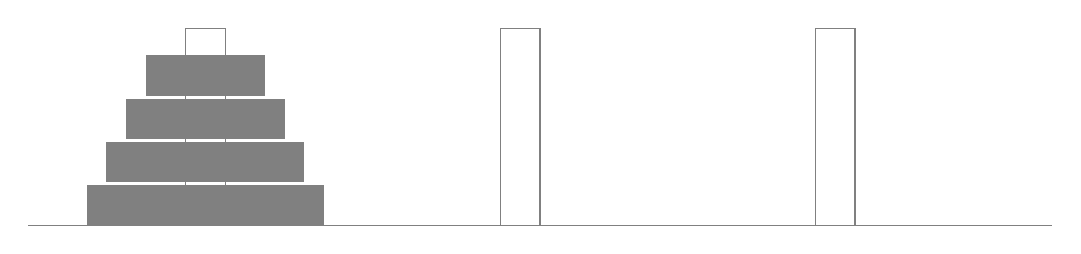
\begin{tikzpicture}[scale=0.5]
	\draw[gray, thin] (0,0) -- (26,0);
	\draw[gray, thin] (4,0) -- (4,5) -- (5,5) -- (5,0);
	\draw[gray, thin] (12,0) -- (12,5) -- (13,5) -- (13,0);
	\draw[gray, thin] (20,0) -- (20,5) -- (21,5) -- (21,0);

	\draw[gray, thin, fill=black!50] (1.5,0) -- (7.5,0) -- (7.5,1) -- (1.5,1) -- cycle;	
	\draw[gray, thin, fill=black!50] (2,1.1) -- (7,1.1) -- (7,2.1) -- (2,2.1) -- cycle;	
	\draw[gray, thin, fill=black!50] (2.5,2.2) -- (6.5,2.2) -- (6.5,3.2) -- (2.5,3.2) -- cycle;	
	\draw[gray, thin, fill=black!50] (3,3.3) -- (6,3.3) -- (6,4.3) -- (3,4.3) -- cycle;
\end{tikzpicture}

\end{center}

\end{problem}

\begin{problem}{4}
	W przestrzeni danych jest $n \geqslant 3$ punktów, że żadne trzy z nich nie leżą na jednej prostej. Każde dwa z tych punktów połączono odcinkiem o kolorze zielonym lub czerwonym. Wykazać, że można wybrać tak jeden z tych kolorów, aby każde dwa z danych punktów były połączone odcinkiem lub łamaną tego koloru.
\end{problem}

\begin{problem}{5} 
Dany jest ciąg liczb rzeczywistych
\[
	a_0 \neq 0, 1,\quad a_1 = 1 - a_0,\quad a_{n + 1} = 1 - a_n(1 - a_n). 
\]
Wykazać, że dla wszystkich $n$ 
\[
	a_1a_2...a_n\left(\frac{1}{a_1} + \frac{1}{a_2} + ... + \frac{1}{a_n}\right) = 1.
\]
\end{problem}

\newpage

\begin{problem}{6} 
	Wykazać, że planszę o wymiarach $2^n \times 2^n$ dla pewnego $n \geqslant 1$ z usuniętym jednym z rogów da się przykryć pewną liczbą L-klocków (takich jak na rysunku). Klocki można obracać.

	\begin{center}
		\begin{tikzpicture}[scale=0.5]
	    \tkzDefPoint(0,0){v_1}
	    \tkzDefPoint(2,0){v_2}
	    \tkzDefPoint(2,2){v_3}
	    \tkzDefPoint(1,2){v_4}
	    \tkzDefPoint(1,1){v_5}
	    \tkzDefPoint(0,1){v_6}
	    \tkzDefPoint(1,0){A}
	    \tkzDefPoint(2,1){B}

	    \tkzDrawSegments(v_1,v_2 v_2,v_3 v_3,v_4 v_4,v_5 v_5,v_6  v_6,v_1)
	    \tkzDrawSegments(v_5,A)
	    \tkzDrawSegments(v_5,B)
		\end{tikzpicture}
	\end{center}
\end{problem}

\begin{problem}{7}
Niech $n$ będzie nieparzystą liczbą naturalną, a liczby $x_1,\; x_2,\; ...,\; x_n$ będą parami różne. Dla każdych dwóch liczb $x_i$ oraz $x_j$, gdzie $i > j$, zapisano na tablicy wartość bezwzględną ich różnicy. Wykazać, że można podzielić zapisane liczby na dwa zbiory o równej sumie.
\end{problem}

